\section{Distribution of Predicted Gene Lengths}

To better understand and compare the distributions of gene lengths
predicted by Braker2, GeneMark, and RefSeq, the cumulative density
function for the lengths of CDS sequences for each gene finding tool
are plotted in figure ~\ref{fig:cdf-lengths}. The log base 10 values
of gene lengths were used for a better visulazation of the
distributions. In DC1, the curves from Braker and GeneMark follow each
other closely, with the only variation being genes of short length,
where Braker's curve extends beyond that of GeneMark, indicating that
Braker predicts more shorter genes than GeneMark. In the case of
Tsth20, the curves are nearly identical. In \textit{T. reesei}, we see
disagreement in the curves for shorter genes, with Braker appearing to
predict a greater amount of shorter genes than GeneMark and
RefSeq. The upper portions of the curve trend towards agreement
between the curves. In \textit{T. harzianum}, RefSeq deviates from
GeneMark and Braker, predicting more genes of short length, while
Braker and GeneMark appear to be in near-complete agreement. Finally,
in \textit{T. virens}, we see the RefSeq curve predicting shorter
genes once again, although the deviation is not as drastic as in
\textit{T. harzianum}. From these plots, we can say that visually,
gene finding tools appear to predict different lengths of genes.

\begin{figure}
  \centering
  \begin{subfigure}{0.7\textwidth}
    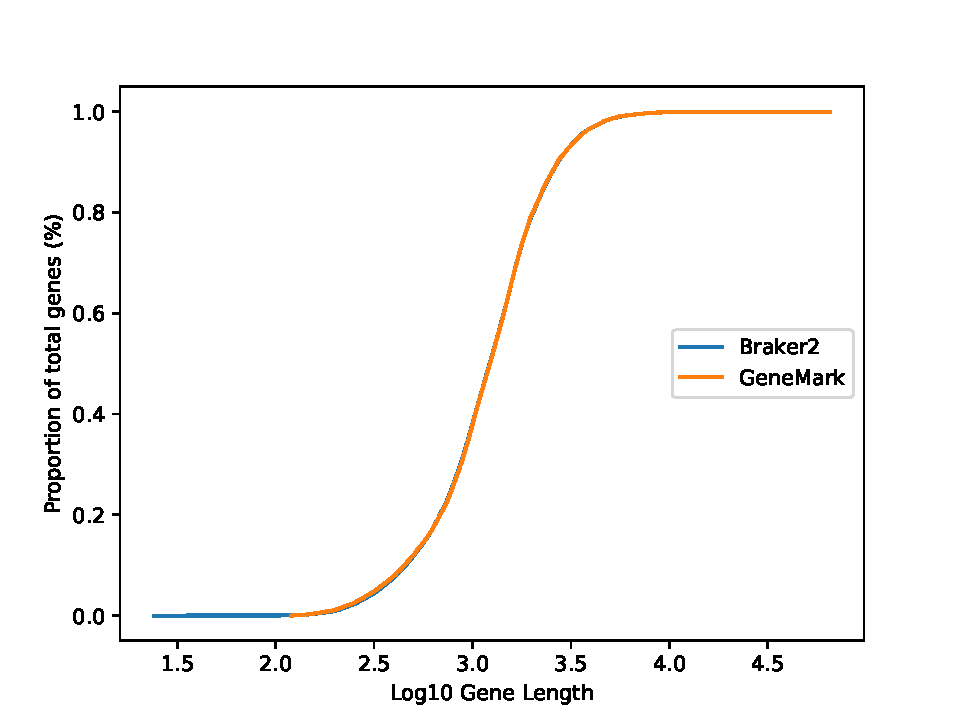
\includegraphics[width=\textwidth]{figures/dc1-cdf-lengths-log.pdf}
    \label{fig:dc1-lengths}
    \caption{DC1}
  \end{subfigure}
  \begin{subfigure}{0.7\textwidth}
    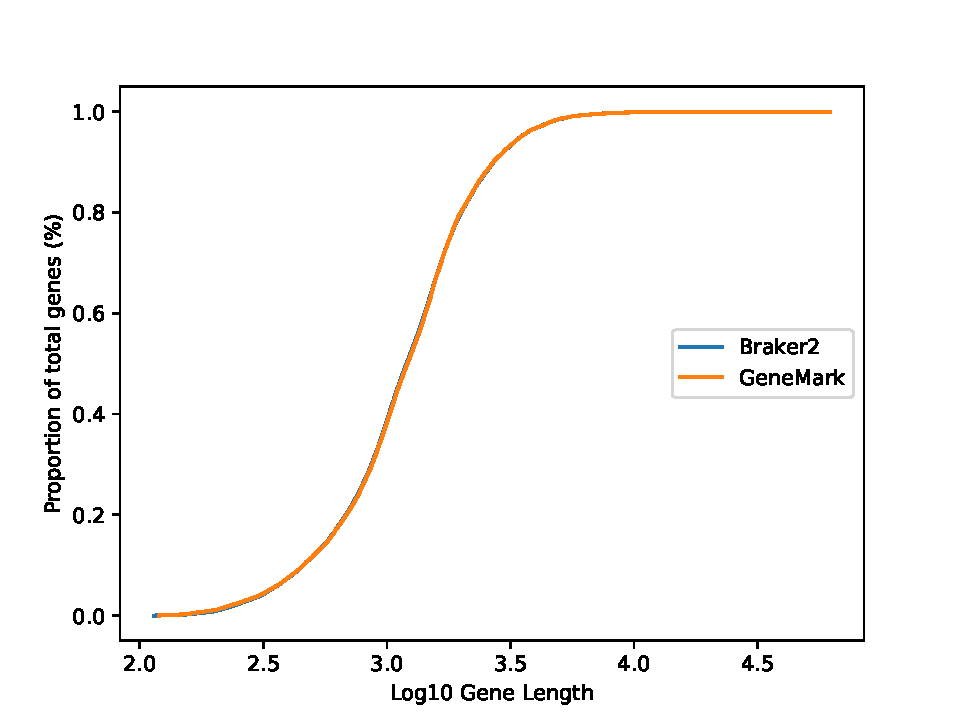
\includegraphics[width=\textwidth]{figures/tsth20-cdf-lengths-log.pdf}
    \label{fig:tsth20-lengths}
    \caption{Tsth20}
  \end{subfigure}
\end{figure}
\begin{figure}
  \ContinuedFloat
  \centering
  \begin{subfigure}{0.7\textwidth}
    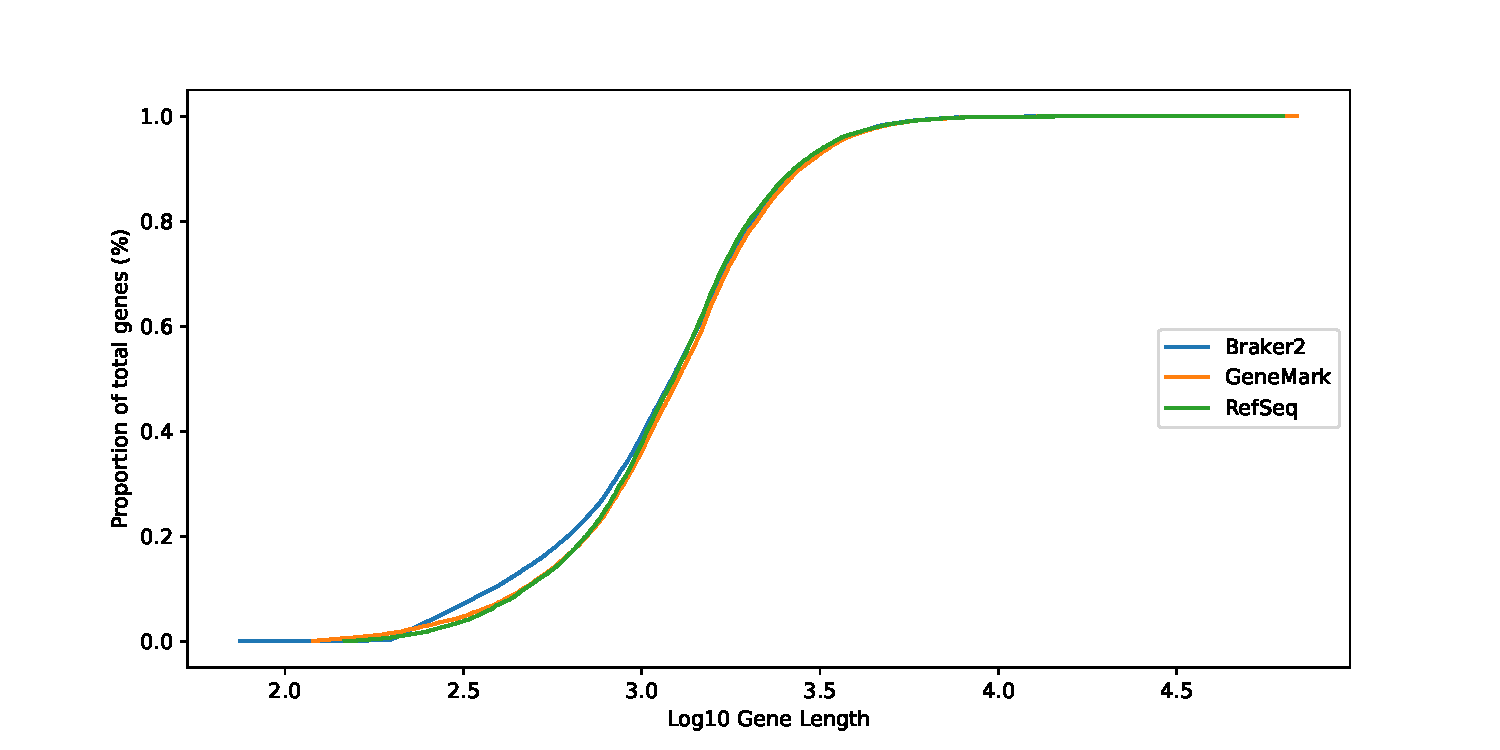
\includegraphics[width=\textwidth]{figures/t-reesei-cdf-lengths-log.pdf}
    \label{fig:treesei-lengths}
    \caption{\textit{T. reesei}}
  \end{subfigure}
  \begin{subfigure}{0.7\textwidth}
    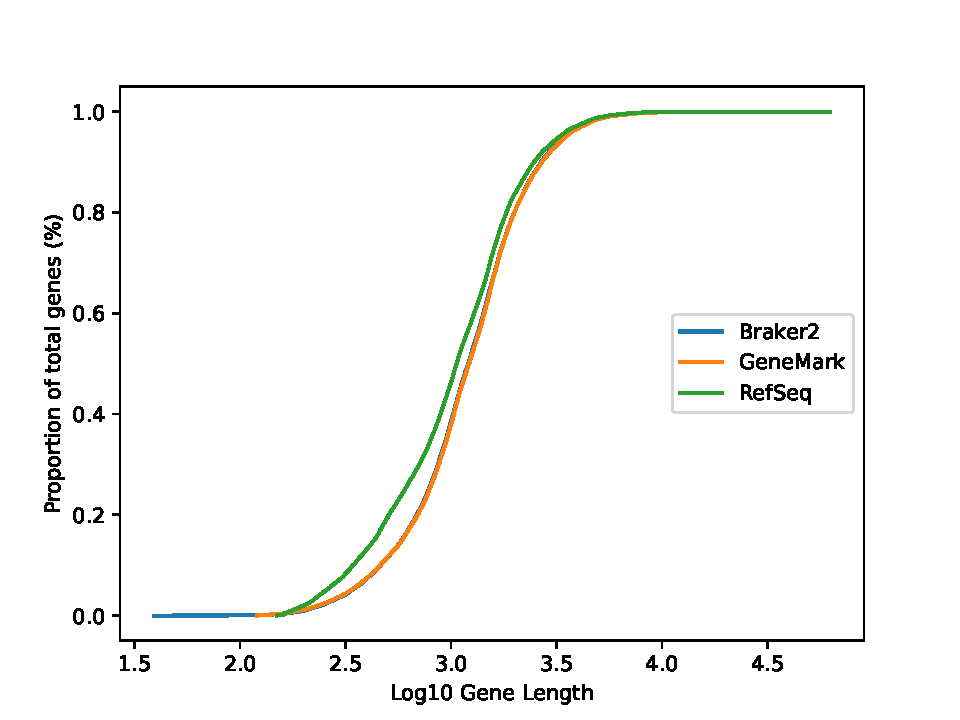
\includegraphics[width=\textwidth]{figures/t-harzianum-cdf-lengths-log.pdf}
    \label{fig:tharzianum-lengths}
    \caption{\textit{T. harzianum}}
  \end{subfigure}
\end{figure}
\begin{figure}
  \ContinuedFloat
  \centering
  \begin{subfigure}{0.7\textwidth}
    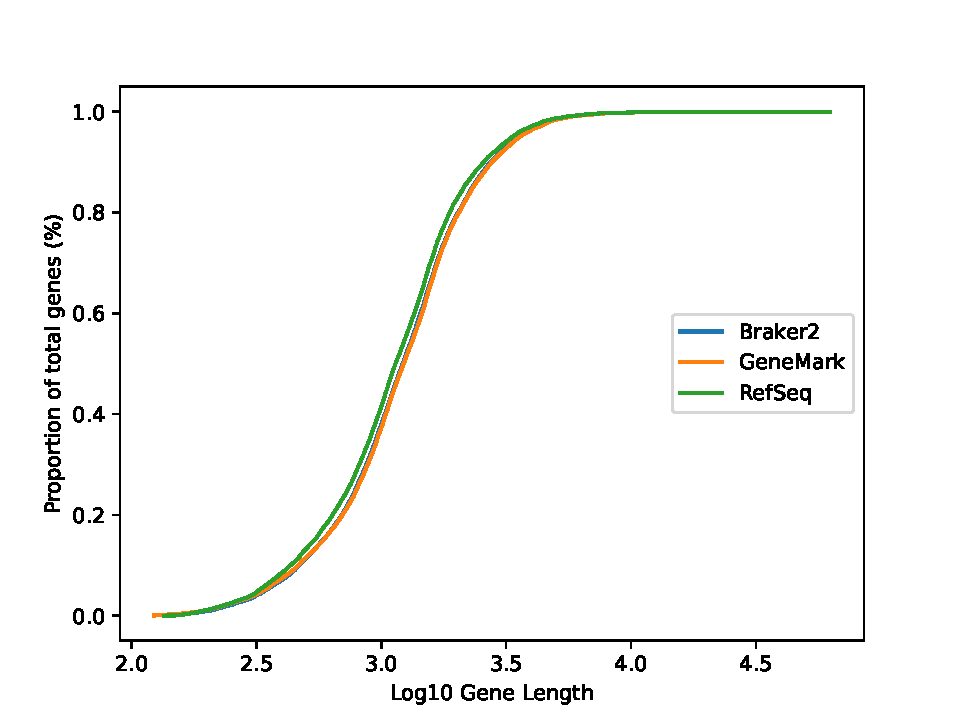
\includegraphics[width=\textwidth]{figures/t-virens-cdf-lengths-log.pdf}
    \label{fig:tvirens-lengths}
    \caption{\textit{T. virens}}
  \end{subfigure}
  \label{fig:cdf-lengths}
  \caption[Cumulative Density Function of Gene Lengths]{Plots of the
    cumulative density function for CDS lengths predicted by each gene
    finding tool.}
\end{figure}

To confirm this statistically, two-sided two-sample Kolmogorov-Smirnov
tests were performed using the log10 transformed gene lengths and are
presented in table \ref{table:ks-2s}. In the cases of DC1 and Tsth20,
we see that Braker and GeneMark do not produce statistically different
lengths of genes. In \textit{T. reesei}, while RefSeq and GeneMark do
not reject the null hypothesis when compared, Braker gene lengths are
significantly different than both RefSeq and GeneMark, which is also
confirmed visually in the CDF plots above. The same cannot be said for
\textit{T. harzianum}, where RefSeq is significantly different from
both GeneMark and Braker, which are not significantly different from
eachother. This observation extends to \textit{T. virens}.

\begin{table}
  \begin{center}
    \begin{tabular}{|c|c|c|c|c|c|c|}
      \hline
      Genome & Tool \#1 & Tool \#2 & \textit{P}-value  \\ \hline
      DC1 & Braker & GeneMark & $0.999$ \\ \hline
      Tsth20 & Braker & GeneMark & $0.965$ \\ \hline
      \textit{T. reesei} & Braker & GeneMark & $9.481^{-07}$ \\ \hline
      \textit{T. reesei} & GeneMark & RefSeq & $0.002$ \\ \hline
      \textit{T. reesei} & Braker & RefSeq & $1.340^{-07}$ \\ \hline
      \textit{T. harzianum} & Braker & GeneMark & $0.863$ \\ \hline
      \textit{T. harzianum} & GeneMark & RefSeq & $4.313^{-52}$ \\ \hline
      \textit{T. harzianum} & Braker & RefSeq & $4.674^{-55}$ \\ \hline
      \textit{T. virens} & Braker & GeneMark & $0.635$ \\ \hline
      \textit{T. virens} & GeneMark & RefSeq & $7.352^{-12}$ \\ \hline
      \textit{T. virens} & Braker & RefSeq & $1.794^{-09}$ \\ \hline
    \end{tabular}
  \end{center}
  \caption{Table of \textit{P}-values from two-sided two-sample
    Kolmogorov-Smirnov tests between gene finding tools.}
  \label{table:ks-2s}
\end{table}

It can clearly be stated that these gene finding tools predict
different lengths of genes, paritcularly in \textit{T. reesei,
  harzianum and virens}. Why that may be the case is a tricky question
to answer without deeper invesitgation. With hesitance, one can make
an observation that when gene finders are applied to the assemblies
from which their training data originated, the gene finders tend to
predict shorter genes.
